%%%%%%%%%%%%%%%%%%%%%%%%%%%%%%%%%%%%%%%%%%%%%%%%%%%%%%%%%%%%%%%%%%%%%%%%
\chapter{Results} \label{chap:Results}
%%%%%%%%%%%%%%%%%%%%%%%%%%%%%%%%%%%%%%%%%%%%%%%%%%%%%%%%%%%%%%%%%%%%%%%%
\vspace{1cm}

In this chapter are exposed the main results obtained from the experiments described in Chapter \ref{chap:Methods}. The analysis focuses on comparing the performance of the three investigated models, which differ in their data augmentation (DA) strategies: the nnU-Net default DA (baseline), the GIN-IPA augmentation, and a combination of both.

First, is reported the overall performance of the models across datasets---Kispi-mial, Kispi-irtk and dHCP---and labels---cerebrospinal fluid (CSF), cortical gray matter (cGM), white matter (WM), ventricles, cerebellum, deep gray matter (dGM) and brainstem (BS). [...]

\section{General Performance} \label{sec:GeneralPerformance}
In the plots below is shown the Dice score (DSC) across datasets and labels for the three models. The model predictions are realized on the test set of the same dataset the model was trained on (in-domain), and on the whole set (both train and test) of the other datasets (out-of-domain, OOD).

To avoid occupying the pages below with too many figures and considering that the general performance of the tested model is well captured with the DSC, here only the plots relative to this metric are shown. Plots regarding volume similarity (VS) and Hausdorff distance 95\th percentile (HD95) are in Appendix \hyperref[app:SupplementaryPlots]{A}.

For the baseline model (see Fig.\,\ref{fig:default_DC}), the drop in performance between in-domain and OOD is clear in every case, except in the DSC of some labels (CSF, cGM, WM and cerebellum) for the model trained on Kispi-mial. The drop is especially evident for the models trained on the Kispi datasets when applied to dHCP. Ventricles are the most affected, but also dGM and WM. The change of domain does not have the same effect on the network trained on Kispi-mial as it has on the other two. This is partially due to the quality of the images in Kispi-mial, which is worse than the others\,\cite{FeTA2022_review}. It is expected that any model evaluated OOD on Kispi-mial will perform worse compared to the other datasets.

\begin{figure}[htbp]
    \centering
    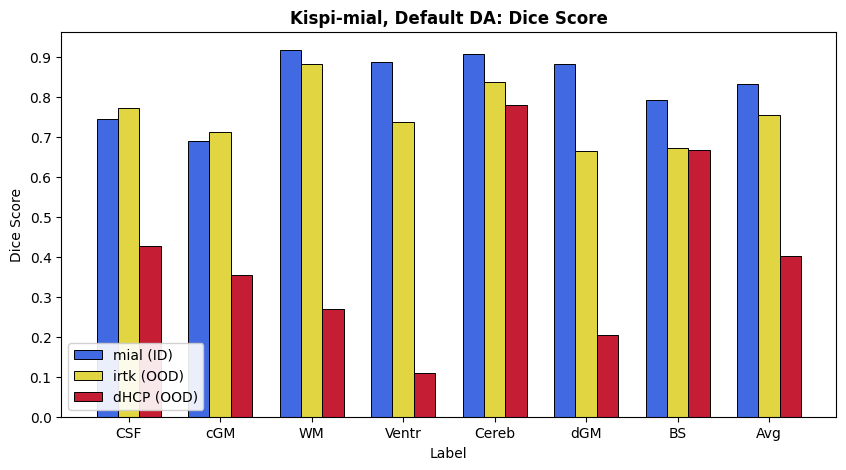
\includegraphics[width=0.8\textwidth]{figures/mial_default_DC.png}\\
    \vspace{10pt}
    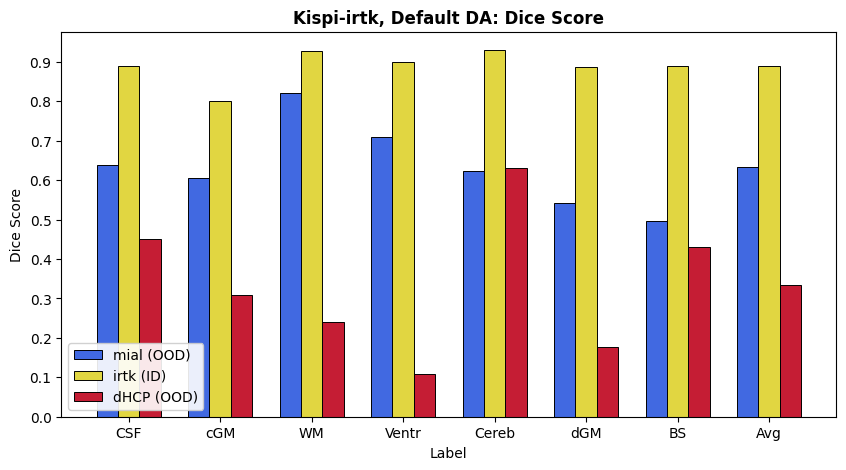
\includegraphics[width=0.8\textwidth]{figures/irtk_default_DC.png}\\
    \vspace{10pt}
    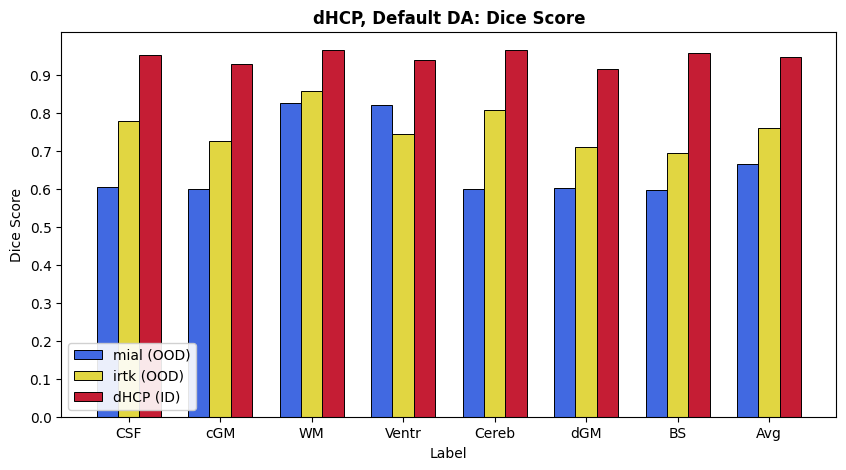
\includegraphics[width=0.8\textwidth]{figures/dHCP_default_DC.png}
    \caption{Dice score across datasets and labels for the nnU-Net default DA (baseline model). From top to bottom: training on Kispi-mial, on Kispi-irtk, and on dHCP.}
    \label{fig:default_DC}
\end{figure}

Although GIN-IPA (see Fig.\,\ref{fig:ginipa_DC}) does not cause an increment in DSC in the models trained on Kispi-mial and dHCP, it produces a significant improvement in the model trained on Kispi-irtk when predicting on dHCP. The raise is mainly located in dGM, ventricles and BS. The average Dice passes from \numrange{0.33}{0.55} (\qty{+66}{\percent}).

\begin{figure}[htbp]
    \centering
    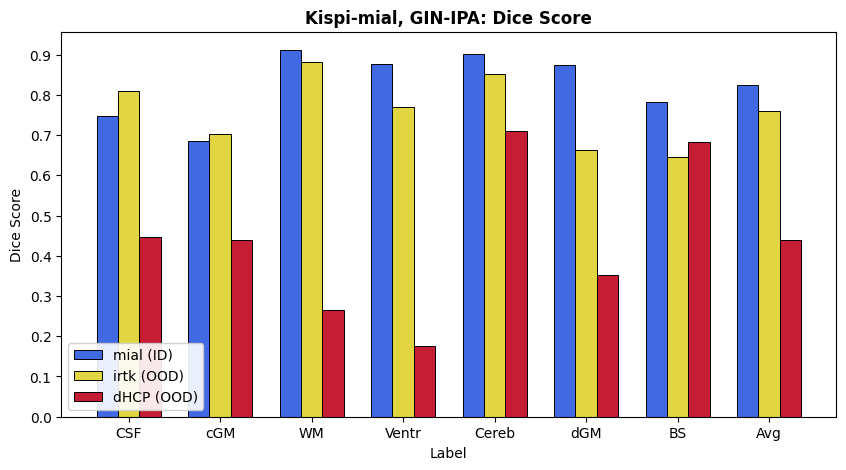
\includegraphics[width=0.8\textwidth]{figures/mial_ginipa_DC.png}\\
    \vspace{10pt}
    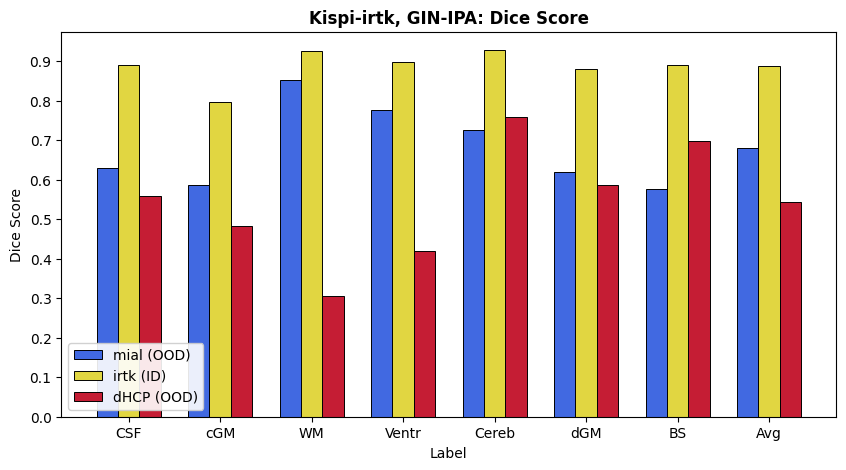
\includegraphics[width=0.8\textwidth]{figures/irtk_ginipa_DC.png}\\
    \vspace{10pt}
    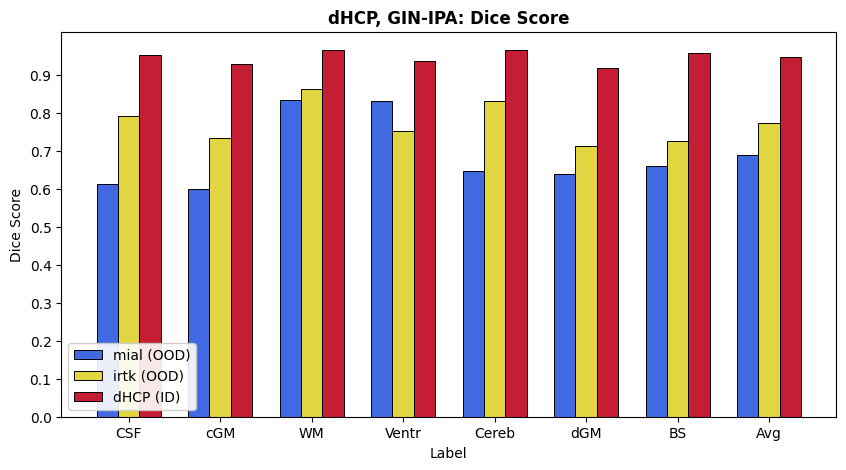
\includegraphics[width=0.8\textwidth]{figures/dHCP_ginipa_DC.png}
    \caption{Dice score across datasets and labels for the GIN-IPA DA model. From top to bottom: training on Kispi-mial, on Kispi-irtk, and on dHCP.}
    \label{fig:ginipa_DC}
\end{figure}

Finally, the model that combines the nnU-Net default DA and GIN-IPA is substantially equivalent to the pure GIN-IPA model (see Fig.\,\ref{fig:both_DC}).

\begin{figure}[htbp]
    \centering
    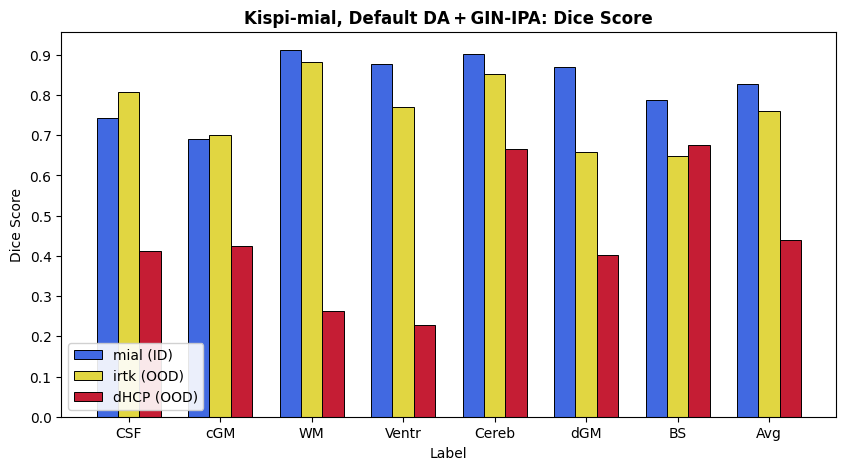
\includegraphics[width=0.8\textwidth]{figures/mial_both_DC.png}\\
    \vspace{10pt}
    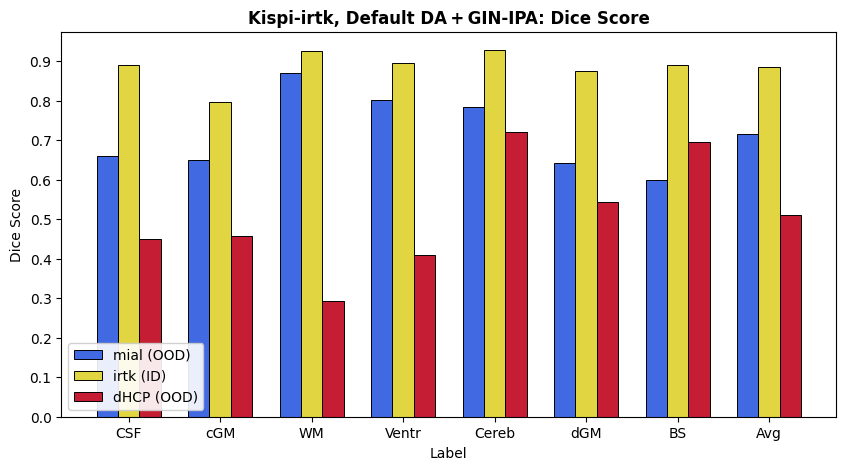
\includegraphics[width=0.8\textwidth]{figures/irtk_both_DC.png}\\
    \vspace{10pt}
    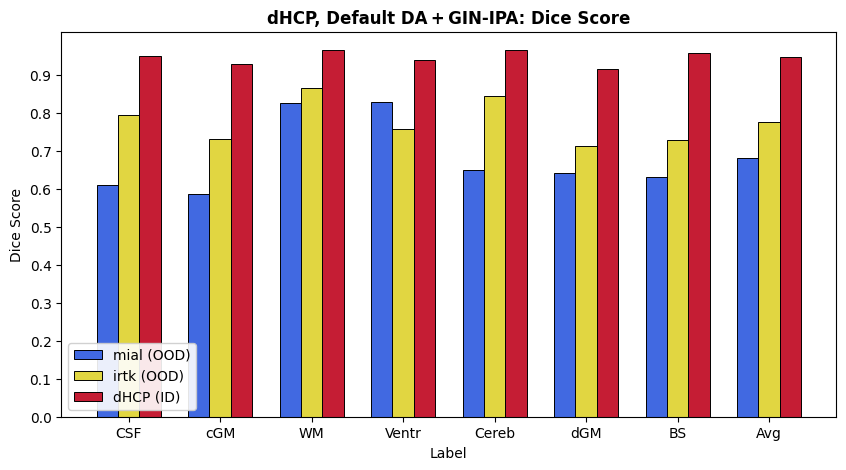
\includegraphics[width=0.8\textwidth]{figures/dHCP_both_DC.png}
    \caption{Dice score across datasets and labels for the combined DA (default\,+\,GIN-IPA) model. From top to bottom: training on Kispi-mial, on Kispi-irtk, and on dHCP.}
    \label{fig:both_DC}
\end{figure}

\section{Method Comparison} \label{sec:MethodComparison}
In order to assess the relative contribution of the proposed augmentation strategies, a pairwise comparison between models was conducted. Specifically, two sets of comparisons were designed:
\begin{itemize}
    \item the nnU-Net baseline with default data augmentation versus the GIN-IPA DA model
    \item the GIN-IPA DA model versus the combined strategy including both default and GIN-IPA augmentations
\end{itemize}
For each of the three evaluation metrics---DSC, VS, and HD95---the distributions of performance values were analyzed. Comparisons were carried out both at the level of individual anatomical structures and for the total average across labels.

Kernel density estimation (KDE) plots were generated for each metric and label, separately for the two model pairs under comparison. Beyond visual inspection, statistical analyses were employed to quantify the significance and magnitude of the observed differences. The Wilcoxon signed-rank test was used to test the null hypothesis of equal paired performance between models. Corresponding \textit{p}-values were computed to assess whether the proposed augmentation strategy led to statistically significant improvements. Besides, Cohen's \textit{d} was computed to quantify the magnitude of the improvement. Following conventional thresholds, \numlist{0.2; 0.5; 0.8} correspond to small, medium, and large effects, respectively. See Section \ref{sec:StatisticalPerformanceAssessment} for more details about the aforementioned tools.

\paragraph{Baseline vs.\ GIN-IPA}
\begin{itemize}
    \item \textbf{Train on Kispi-mial}
    \begin{itemize}
        \item \textbf{Inference on Kispi-mial:} no measurable difference across metrics and labels; KDE curves largely overlap.
        \item \textbf{Inference on Kispi-irtk:} CSF improves in DSC, VS, and HD95; ventricles improve in DSC and HD95. The pattern reflects heavy failures of the baseline on a subset of difficult volumes. \stats{\,}{\,} (CSF); \stats{\,}{\,} (Ventricles).
        \item \textbf{Inference on dHCP:} significant, strong improvements for cGM, dGM, and ventricles in DSC and VS; the overall average shows a significant small gain. \stats{\,}{\,} (cGM); \stats{\,}{\,} (dGM); \stats{\,}{\,} (Ventricles); overall \stats{\,}{\,}.
    \end{itemize}
    \item \textbf{Train on Kispi-irtk}
    \begin{itemize}
        \item \textbf{Inference on Kispi-mial:} significant, moderate improvements for dGM and ventricles across DSC, VS, and HD95; small improvement on the overall average. \stats{\,}{\,} (dGM); \stats{\,}{\,} (Ventricles); overall \stats{\,}{\,}.
        \item \textbf{Inference on Kispi-irtk:} no difference.
        \item \textbf{Inference on dHCP:} significant, strong improvements across all three metrics and tissues; the mean DSC increases from $0.36$ to $0.54$. Overall \stats{\,}{\,}.
    \end{itemize}
    \item \textbf{Train on dHCP}
    No differences observed on any inference dataset, metric, or label.
\end{itemize}

\paragraph{GIN-IPA vs.\ Combined Augmentation}
\begin{itemize}
    \item \textbf{Train on Kispi-mial}
    \begin{itemize}
        \item \textbf{Inference on Kispi-mial:} no difference.
        \item \textbf{Inference on Kispi-irtk:} no difference.
        \item \textbf{Inference on dHCP:} small, significant improvements for ventricles and dGM across DSC, VS, and HD95. \stats{\,}{\,} (Ventricles); \stats{\,}{\,} (dGM).
    \end{itemize}
    \item \textbf{Train on Kispi-irtk}
    \begin{itemize}
        \item \textbf{Inference on Kispi-mial:} moderate, significant improvements for cGM, WM, and cerebellum in DSC and HD95; small improvement on the overall average. \stats{\,}{\,} (cGM); \stats{\,}{\,} (WM); \stats{\,}{\,} (Cerebellum); overall \stats{\,}{\,}.
        \item \textbf{Inference on Kispi-irtk:} no difference.
        \item \textbf{Inference on dHCP:} combined augmentation performs significantly worse than GIN-IPA alone, especially for CSF, cerebellum, and dGM across metrics. \stats{\,}{\,} (CSF); \stats{\,}{\,} (Cerebellum); \stats{\,}{\,} (dGM).
    \end{itemize}
    \item \textbf{Train on dHCP}
    No differences observed on any inference dataset, metric, or label.
\end{itemize}

\begin{table}[htbp]
    \centering
    \begin{tabular}{c|c|c|c|c|c}
        \toprule
        \textbf{Train DS} & \textbf{Inference DS} & \textbf{Metric} & \textbf{\textit{p}-value} & \textbf{Cohen's \textit{d}} & \textbf{Samples} \\
        \midrule
        \multirow{9}{*}{Kispi-mial}
            & \multirow{3}{*}{Kispi-mial} & DSC  &  &  &  \\
            &                             & VS   &  &  &  \\
            &                             & HD95 &  &  &  \\
        \hhline{~-----}
            & \multirow{3}{*}{Kispi-irtk} & DSC  &  &  &  \\
            &                             & VS   &  &  &  \\
            &                             & HD95 &  &  &  \\
        \hhline{~-----}
            & \multirow{3}{*}{dHCP} & DSC  &  &  &  \\
            &                       & VS   &  &  &  \\
            &                       & HD95 &  &  &  \\
        \hline
        \multirow{9}{*}{Kispi-irtk}
            & \multirow{3}{*}{Kispi-mial} & DSC  &  &  &  \\
            &                             & VS   &  &  &  \\
            &                             & HD95 &  &  &  \\
        \hhline{~-----}
            & \multirow{3}{*}{Kispi-irtk} & DSC  &  &  &  \\
            &                             & VS   &  &  &  \\
            &                             & HD95 &  &  &  \\
        \hhline{~-----}
            & \multirow{3}{*}{dHCP} & DSC  &  &  &  \\
            &                       & VS   &  &  &  \\
            &                       & HD95 &  &  &  \\
        \hline
        \multirow{9}{*}{dHCP}
            & \multirow{3}{*}{Kispi-mial} & DSC  &  &  &  \\
            &                             & VS   &  &  &  \\
            &                             & HD95 &  &  &  \\
        \hhline{~-----}
            & \multirow{3}{*}{Kispi-irtk} & DSC  &  &  &  \\
            &                             & VS   &  &  &  \\
            &                             & HD95 &  &  &  \\
        \hhline{~-----}
            & \multirow{3}{*}{dHCP} & DSC  &  &  &  \\
            &                       & VS   &  &  &  \\
            &                       & HD95 &  &  &  \\
        \bottomrule
    \end{tabular}
    \caption{Baseline vs.\ GIN-IPA: Wilcoxon \textit{p}-values and Cohen's \textit{d} across training/inference datasets and metrics. ${ }^{\dagger}$: \textit{p}-value $< 0.05$; ${ }^{\ddagger}$: \textit{p}-value $<0.01$. ${ }^{*}$: $\abs{d}>0.2$; ${ }^{**}$: $\abs{d}>0.5$; ${ }^{***}$: $\abs{d}>0.8$.}
    \label{tab:baseline-vs-ginipa-stats}
\end{table}

\begin{table}[htbp]
  \centering
  \begin{tabular}{c|c|c|c|c|c}
    \toprule
    \textbf{Train DS} & \textbf{Inference DS} & \textbf{Metric} & \textbf{\textit{p}-value} & \textbf{Cohen's \textit{d}} & \textbf{Samples} \\
    \midrule
    \multirow{9}{*}{Kispi-mial}
      & \multirow{3}{*}{Kispi-mial} & DSC  &  &  &  \\
      &                             & VS   &  &  &  \\
      &                             & HD95 &  &  &  \\
    \hhline{~-----}
      & \multirow{3}{*}{Kispi-irtk} & DSC  &  &  &  \\
      &                             & VS   &  &  &  \\
      &                             & HD95 &  &  &  \\
    \hhline{~-----}
      & \multirow{3}{*}{dHCP} & DSC  &  &  &  \\
      &                       & VS   &  &  &  \\
      &                       & HD95 &  &  &  \\
    \hline
    \multirow{9}{*}{Kispi-irtk}
      & \multirow{3}{*}{Kispi-mial} & DSC  &  &  &  \\
      &                             & VS   &  &  &  \\
      &                             & HD95 &  &  &  \\
    \hhline{~-----}
      & \multirow{3}{*}{Kispi-irtk} & DSC  &  &  &  \\
      &                             & VS   &  &  &  \\
      &                             & HD95 &  &  &  \\
    \hhline{~-----}
      & \multirow{3}{*}{dHCP} & DSC  &  &  &  \\
      &                       & VS   &  &  &  \\
      &                       & HD95 &  &  &  \\
    \hline
    \multirow{9}{*}{dHCP}
      & \multirow{3}{*}{Kispi-mial} & DSC  &  &  &  \\
      &                             & VS   &  &  &  \\
      &                             & HD95 &  &  &  \\
    \hhline{~-----}
      & \multirow{3}{*}{Kispi-irtk} & DSC  &  &  &  \\
      &                             & VS   &  &  &  \\
      &                             & HD95 &  &  &  \\
    \hhline{~-----}
      & \multirow{3}{*}{dHCP} & DSC  &  &  &  \\
      &                       & VS   &  &  &  \\
      &                       & HD95 &  &  &  \\
    \bottomrule
  \end{tabular}
  \caption{GIN-IPA vs.\ combined augmentation: Wilcoxon \textit{p}-values and Cohen's \textit{d} across training/inference datasets and metrics. ${ }^{\dagger}$: \textit{p}-value $< 0.05$; ${ }^{\ddagger}$: \textit{p}-value $<0.01$. ${ }^{*}$: $\abs{d}>0.2$; ${ }^{**}$: $\abs{d}>0.5$; ${ }^{***}$: $\abs{d}>0.8$.}
  \label{tab:comparison_2}
\end{table}
